\chapter{Resultados}
\label{chap:resultados}

\noindent Este cap├¡tulo presenta los hallazgos emp├¡ricos del estudio, siguiendo la secuencia metodol├│gica establecida. Iniciamos con la caracterizaci├│n de la cohorte y el an├ílisis de la variabilidad de los datos, lo cual fundamenta las decisiones de preprocesamiento. A continuaci├│n, detallamos el proceso de establecimiento de la ``verdad operativa'' mediante el an├ílisis de conglomerados. Posteriormente, presentamos el rendimiento del sistema de inferencia difusa en su validaci├│n contra esta referencia. Finalmente, exponemos un an├ílisis de robustez que revela la contribuci├│n sin├®rgica de las variables al modelo.

% ============================================================================
\section{Caracterización de la Cohorte y Análisis de Variabilidad de Datos}
\label{sec:caracterizacion_cohorte}
% ============================================================================

La cohorte final del estudio estuvo compuesta por 10 participantes adultos (5 mujeres, 5 hombres) con un seguimiento longitudinal multianual, acumulando un total de 9,185 d├¡as de registro. Un an├ílisis de variabilidad dual se llev├│ a cabo para cuantificar la dispersi├│n de las m├®tricas biom├®tricas tanto en su estado observado (sin imputaciones) como operativo (post-imputaci├│n).

Se encontr├│ una heterogeneidad considerable tanto inter-sujeto (entre diferentes participantes) como intra-sujeto (en el d├¡a a d├¡a de un mismo participante). El coeficiente de variaci├│n (CV) para m├®tricas clave como los minutos de ejercicio diario super├│ el 100\%, lo cual indica una alta irregularidad en los patrones de actividad incluso despu├®s de la imputaci├│n jer├írquica. Este comportamiento motiv├│ el uso de estad├¡sticos robustos (mediana e IQR) y fundamenta la interpretaci├│n posterior de los perfiles detectados mediante clustering.

Como observamos, algunos usuarios exhiben patrones más consistentes (CV más bajos) que otros. Esta alta variabilidad natural de los datos recopilados en condiciones de vida libre justificó la decisión metodológica de agregar los datos a nivel semanal utilizando estadísticos robustos (mediana e IQR), con el fin de amortiguar el ruido diario y analizar patrones de comportamiento más estables y sostenidos.

% ============================================================================
\section{Establecimiento de la Verdad Operativa: Análisis de Conglomerados}
\label{sec:verdad_operativa_clustering}
% ============================================================================

Previo al análisis de conglomerados, se verificó la ausencia de multicolinealidad severa entre las ocho características semanales seleccionadas. La \Cref{fig:matriz_correlacion} muestra la matriz de correlación de Pearson entre variables: todas presentaron un Factor de Inflación de la Varianza (VIF) inferior a 2.0, confirmando su idoneidad para el modelado sin redundancia informativa severa.

\begin{figure}[htbp]
    \centering
    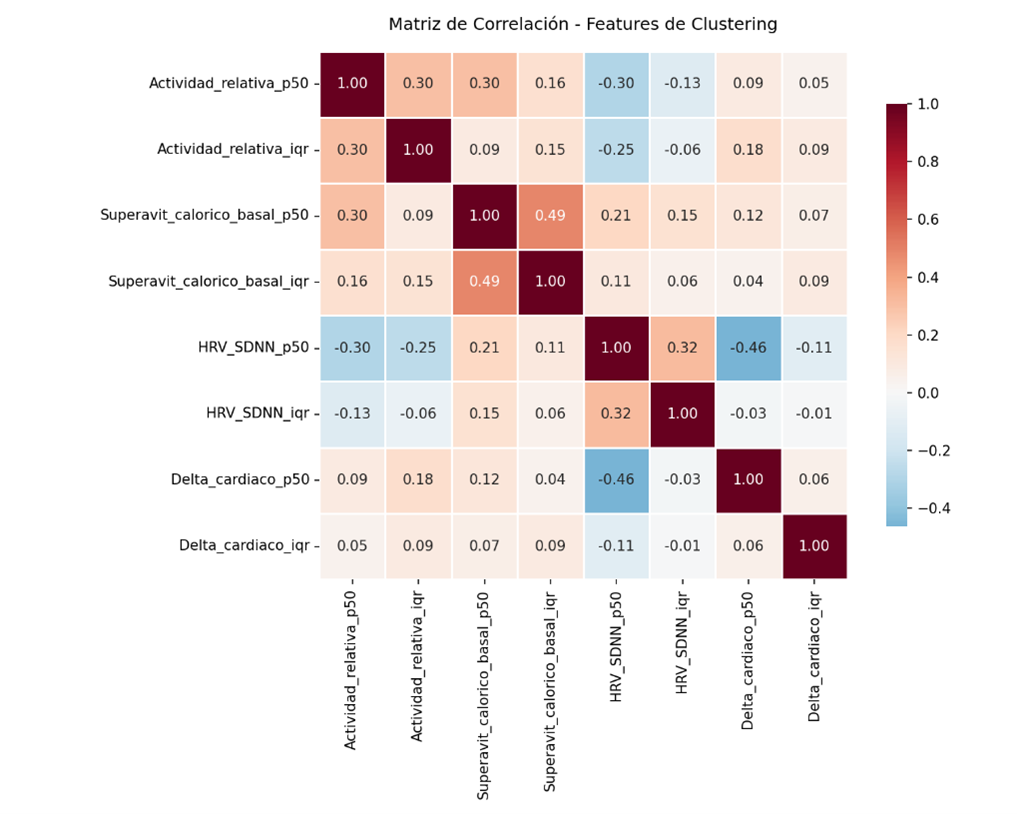
\includegraphics[width=0.85\textwidth]{figuras/matriz_correlacion_features_clustering.png}
    \caption{Matriz de correlación de características para clustering}
    \label{fig:matriz_correlacion}
\end{figure}

Posteriormente, realizamos un barrido de $K$ (de 2 a 6 conglomerados) para determinar la partici├│n m├ís adecuada de los datos. Como observamos en la \Cref{fig:silhouette_elbow}, el coeficiente de Silhouette alcanz├│ su m├íximo en $K=2$ (S=0.232), lo que indica que la estructura m├ís clara y estable en los datos correspond├¡a a dos perfiles de comportamiento distintos. El m├®todo del codo complement├│ esta decisi├│n mostrando una inflexi├│n en $K=2$.

\begin{figure}[htbp]
    \centering
    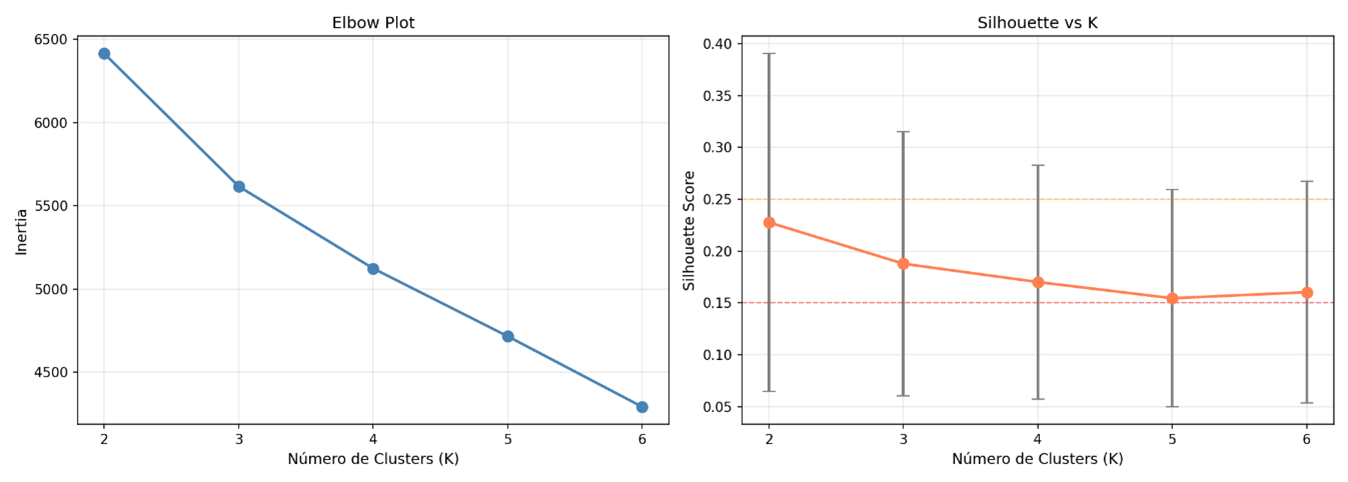
\includegraphics[width=0.9\textwidth]{figuras/PCA_elbow_vs_shilloete.png}
    \caption{Determinaci├│n de K ├│ptimo mediante Silhouette y m├®todo del codo}
    \label{fig:silhouette_elbow}
\end{figure}

El análisis de componentes principales (PCA) confirmó visualmente esta estructura bimodal. La \Cref{fig:pca_biplot} muestra la proyección de las semanas en el espacio reducido de dos componentes principales: el PC1 (37\% de varianza explicada) separa claramente los dos grupos, estando fuertemente influenciado por las variables de actividad y gasto calórico.

\begin{figure}[htbp]
    \centering
    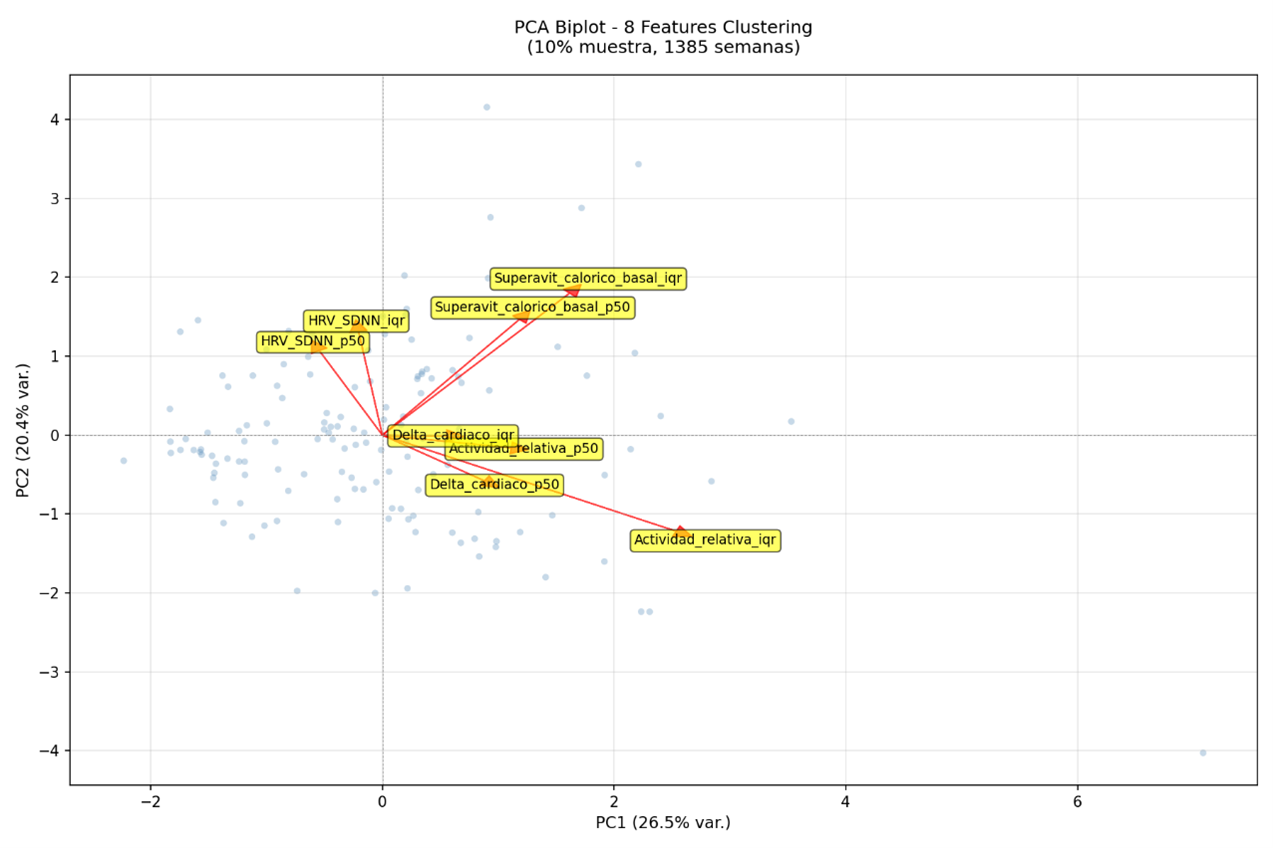
\includegraphics[width=0.95\textwidth]{figuras/PCA_biplot.png}
    \caption{Biplot de componentes principales mostrando separaci├│n bimodal}
    \label{fig:pca_biplot}
\end{figure}

Los perfiles de estos dos conglomerados se analizaron estadísticamente para su caracterización clínica. Como ilustra la \Cref{fig:perfiles_clusters}, el Conglomerado 0 (``Bajo Sedentarismo'') presentó valores de mediana significativamente más altos en Actividad\_relativa\_p50 y Superavit\_calorico\_basal\_p50 en comparación con el Conglomerado 1 (``Alto Sedentarismo''). Las diferencias fueron estadísticamente irrefutables ($p < .001$) y con un tamaño del efecto grande (Cohen's $d > 0.9$). Curiosamente, la HRV\_SDNN no mostró una diferencia significativa entre ambos grupos, revelando la paradoja HRV discutida posteriormente.

\begin{figure}[htbp]
    \centering
    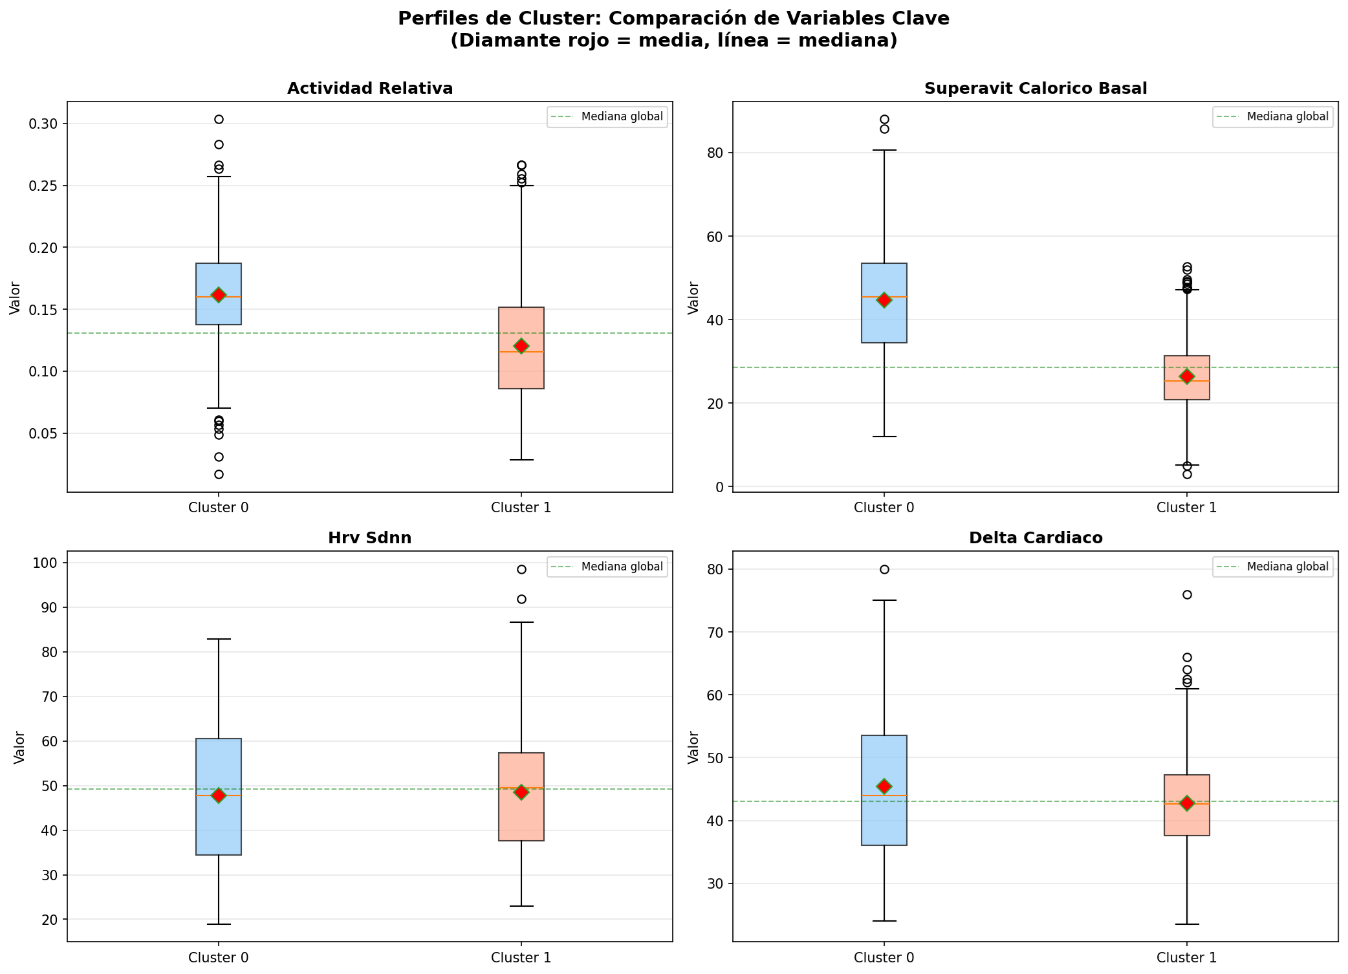
\includegraphics[width=0.95\textwidth]{figuras/perfiles_de_clusters.png}
    \caption{Perfiles biom├®tricos de los dos conglomerados identificados}
    \label{fig:perfiles_clusters}
\end{figure}

La \Cref{tab:distribucion_clusters_usuario} muestra la distribuci├│n de semanas asignadas a cada conglomerado por usuario.

\begin{table}[htbp]
\centering
\caption{Distribuci├│n de Semanas por Conglomerado y Usuario}
\label{tab:distribucion_clusters_usuario}
\small
\begin{tabular}{@{}lcccr@{}}
\toprule
\textbf{Usuario} & \textbf{Cluster Alto Sed (\%)} & \textbf{Cluster Bajo Sed (\%)} & \textbf{Diferencia absoluta (\%)} \\
\midrule
u1  & 99.3 & 0.7  & 98.7 \\
u2  & 85.7 & 14.3 & 71.4 \\
u3  & 11.3 & 88.7 & 77.3 \\
u4  & 71.4 & 28.6 & 42.9 \\
u5  & 64.3 & 35.7 & 28.6 \\
u6  & 82.0 & 18.0 & 64.0 \\
u7  & 94.7 & 5.3  & 89.5 \\
u8  & 27.7 & 72.3 & 44.5 \\
u9  & 84.2 & 15.8 & 68.5 \\
u10 & 80.9 & 19.1 & 61.8 \\
\bottomrule
\end{tabular}
\end{table}

La asignación de cada una de las 1,337 semanas válidas a uno de estos dos conglomerados se constituyó como la ``verdad operativa'': una clasificación objetiva y empírica utilizada como referencia para la validación del sistema de inferencia difusa.

% ============================================================================
\section{Rendimiento del Sistema de Inferencia Difusa}
\label{sec:rendimiento_sistema_difuso}
% ============================================================================

El rendimiento del modelo difuso se evalu├│ mediante su concordancia con la clasificaci├│n de la verdad operativa. Tras una b├║squeda del umbral de decisi├│n ($\tau$) que maximizara el F1-Score, se estableci├│ un valor ├│ptimo de $\tau = 0.30$. Con este umbral, el sistema difuso alcanz├│ un rendimiento global robusto, con un F1-Score de 0.840, una Exactitud de 0.740 y una alta Sensibilidad (Recall) de 0.976.

El análisis por participante reveló una heterogeneidad en el rendimiento, con un F1-Score que osciló entre 0.215 y 0.997. Usuarios con patrones de comportamiento más estables mostraron una concordancia muy alta (ej. u1, u7), mientras que aquellos con mayor variabilidad intra-semanal presentaron mayores discrepancias. Estos resultados evidencian áreas de oportunidad para la personalización futura del modelo.

La \Cref{tab:rendimiento_louo} presenta los resultados de la validaci├│n cruzada Leave-One-User-Out (LOUO) por usuario.

% Tabla multi-página con longtable
\begin{longtable}{@{}lcccccccccccc@{}}
\caption{Rendimiento del Sistema Difuso por Usuario (Validaci├│n LOUO)}
\label{tab:rendimiento_loou} \\
\toprule
\textbf{Usuario} & \textbf{Semanas} & \textbf{\% Obs.*} & \textbf{Acc} & \textbf{Prec} & \textbf{Rec} & \textbf{F1} & \textbf{MCC} & \textbf{$\tau$} & \textbf{TP} & \textbf{FP} & \textbf{TN} & \textbf{FN} \\
\midrule
\endfirsthead
\multicolumn{13}{c}{\tablename\ \thetable{} -- continuaci├│n} \\
\toprule
\textbf{Usuario} & \textbf{Semanas} & \textbf{\% Obs.*} & \textbf{Acc} & \textbf{Prec} & \textbf{Rec} & \textbf{F1} & \textbf{MCC} & \textbf{$\tau$} & \textbf{TP} & \textbf{FP} & \textbf{TN} & \textbf{FN} \\
\midrule
\endhead
\midrule
\multicolumn{13}{r}{Continúa en la siguiente página} \\
\endfoot
\bottomrule
\endlastfoot
u1  & 159 & 100 & 0.987 & 0.987 & 1.000 & 0.994 & 0.000 & 0.2 & 157 & 2   & 0  & 0 \\
u2  & 8   & 100 & 0.500 & 0.800 & 0.571 & 0.667 & -0.293 & 0.2 & 4   & 1   & 0  & 3 \\
u3  & 141 & 100 & 0.397 & 0.432 & 0.739 & 0.545 & 0.076 & 0.1 & 51  & 67  & 5  & 18 \\
u4  & 15  & 100 & 0.733 & 0.733 & 1.000 & 0.846 & 0.302 & 0.4 & 11  & 4   & 0  & 0 \\
u5  & 15  & 100 & 0.733 & 0.714 & 1.000 & 0.833 & 0.000 & 0.4 & 10  & 4   & 1  & 0 \\
u6  & 303 & 100 & 0.515 & 0.513 & 0.994 & 0.677 & 0.093 & 0.1 & 154 & 146 & 2  & 1 \\
u7  & 117 & 100 & 0.957 & 0.957 & 1.000 & 0.978 & 0.387 & 0.45 & 111 & 5   & 1  & 0 \\
u8  & 192 & 100 & 0.391 & 0.417 & 0.714 & 0.526 & 0.064 & 0.1 & 65  & 91  & 10 & 26 \\
u9  & 302 & 100 & 0.745 & 0.747 & 0.977 & 0.847 & 0.304 & 0.1 & 213 & 72  & 12 & 5 \\
u10 & 133 & 100 & 0.797 & 0.797 & 1.000 & 0.887 & 0.000 & 0.4 & 106 & 27  & 0  & 0 \\
\end{longtable}

\begin{flushleft}
\small
\textit{Nota:} \% Obs.* = Porcentaje de datos observados (sin imputaci├│n). Acc = Accuracy, Prec = Precision, Rec = Recall, MCC = Matthews Correlation Coefficient, $\tau$ = umbral de decisi├│n ├│ptimo, TP = Verdaderos Positivos, FP = Falsos Positivos, TN = Verdaderos Negativos, FN = Falsos Negativos.
\end{flushleft}

\subsection{Posicionamiento en el Contexto de Estudios con Validaci├│n LOUO}
\label{subsec:comparativa_louo}

La \Cref{tab:comparativa_louo} posiciona el desempe├▒o del sistema en el contexto de estudios recientes con cohortes de tama├▒o comparable que emplean validaci├│n LOUO/LOSO (Leave-One-Subject-Out) en dominios de salud con wearables.

\begin{table}[htbp]
\centering
\caption{Comparaci├│n de Validaci├│n LOUO/LOSO en Cohortes Peque├▒as con Wearables (2018-2025)}
\label{tab:comparativa_louo}
\small
\begin{tabular}{@{}llcccc@{}}
\toprule
\textbf{Estudio} & \textbf{Dominio} & \textbf{N} & \textbf{M├®trica} & \textbf{Valor} & \textbf{CV\%} \\
\midrule
Alinia 2020 & Actividad física & 10 & Accuracy & 0.812 & 6.3\% \\
Mullick 2022 & Depresi├│n & 37 & F1-Score & 0.650 & NR \\
Crozat 2025 & Conteo pasos & 7 & MAPE & 13.6\% & NR \\
Ricotti 2023 & Progresi├│n DMD & 21 & R┬▓ & 0.900 & NR \\
Kaveh 2024 & Somnolencia & 9 & Accuracy & 0.933 & NR \\
\midrule
\textbf{Este estudio} & \textbf{Sedentarismo} & \textbf{10} & \textbf{F1-Score} & \textbf{0.780} & \textbf{21.4\%} \\
\bottomrule
\end{tabular}
\begin{flushleft}
\scriptsize
\textit{Nota:} NR = No reportado. DMD = Distrofia Muscular de Duchenne. CV\% = Coeficiente de variaci├│n del desempe├▒o entre folds. Estudios seleccionados por uso de validaci├│n LOUO/LOSO en cohortes N<40.
\end{flushleft}
\end{table}

El F1-Score de 0.780 ± 0.167 (CV=21.4\%) es comparable a los mejores resultados reportados (Kaveh et al., 2024; Ricotti et al., 2023), pero destaca por tres características distintivas:

\begin{enumerate}
    \item \textbf{Generalizaci├│n inter-sujeto robusta:} Con 7 de 10 usuarios alcanzando F1$\geq$0.65, el sistema demuestra capacidad de generalizaci├│n adecuada a pesar de la heterogeneidad conductual inherente a estudios de vida libre. El coeficiente de variaci├│n (CV=21.4\%) refleja variabilidad esperada en cohortes peque├▒as (N=10) con seguimientos heterog├®neos (7-298 semanas por usuario), y es comparable con estudios de validaci├│n de wearables en condiciones ecol├│gicas \cite{Doherty2021}.
    
    \item \textbf{Parsimonia del modelo:} El sistema emplea 4 variables de entrada, significativamente menos que las 10-20 características típicas en la literatura de clasificación de actividad con acelerometría \cite{Alinia2020}. Esta simplicidad facilita interpretabilidad clínica y reducción de costos computacionales.
    
    \item \textbf{Transparencia metodol├│gica:} Reportamos el rendimiento completo (F1-Score ┬▒ SD) por usuario (ver \Cref{tab:rendimiento_louo}), pr├íctica infrecuente en literatura actual. Estudios como Mullick et al. \cite{Mullick2022} y Crozat et al. \cite{Crozat2025} reportan m├®tricas globales sin desglose por participante, limitando la evaluaci├│n de heterogeneidad de respuesta.
\end{enumerate}

Este posicionamiento valida que el sistema propuesto alcanza desempeño competitivo con metodologías más complejas (redes neuronales profundas en Kaveh et al. \cite{Kaveh2024}), preservando la ventaja de interpretabilidad inherente a los sistemas difusos basados en reglas.

La \Cref{tab:caracteristicas_usuario} presenta las caracter├¡sticas biom├®tricas semanales por usuario (mediana $\pm$ desviaci├│n est├índar).

\begin{landscape}
\begin{table}[p]
\centering
\caption{Caracter├¡sticas Biom├®tricas Semanales por Usuario (Mediana $\pm$ DE)}
\label{tab:caracteristicas_usuario}
\tiny
\begin{tabular}{@{}lccccccccc@{}}
\toprule
\textbf{Usuario} & \textbf{Act\_rel\_p50} & \textbf{Act\_rel\_iqr} & \textbf{Sup\_cal\_p50} & \textbf{Sup\_cal\_iqr} & \textbf{HRV\_p50} & \textbf{HRV\_iqr} & \textbf{Delta\_FC\_p50} & \textbf{Delta\_FC\_iqr} & \textbf{Score\_fuzzy} \\
\midrule
u1  & 0.083 ($\pm$0.029) & 0.041 ($\pm$0.027) & 22.839 ($\pm$5.172)  & 9.327 ($\pm$5.760)   & 54.995 ($\pm$6.304) & 11.373 ($\pm$4.877) & 37.046 ($\pm$4.039) & 8.615 ($\pm$4.647)  & 0.644 ($\pm$0.211) \\
u2  & 0.161 ($\pm$0.028) & 0.072 ($\pm$0.043) & 33.069 ($\pm$4.957)  & 16.296 ($\pm$6.997)  & 40.651 ($\pm$6.816) & 7.654 ($\pm$2.997)  & 40.711 ($\pm$4.800) & 9.118 ($\pm$6.176)  & 0.334 ($\pm$0.334) \\
u3  & 0.145 ($\pm$0.049) & 0.096 ($\pm$0.038) & 46.009 ($\pm$11.031) & 25.709 ($\pm$14.350) & 34.696 ($\pm$8.376) & 12.893 ($\pm$7.845) & 57.413 ($\pm$8.047) & 11.451 ($\pm$4.718) & 0.465 ($\pm$0.250) \\
u4  & 0.163 ($\pm$0.057) & 0.089 ($\pm$0.039) & 21.362 ($\pm$6.943)  & 7.941 ($\pm$3.238)   & 38.662 ($\pm$6.757) & 11.192 ($\pm$7.132) & 49.250 ($\pm$4.205) & 12.780 ($\pm$6.044) & 0.719 ($\pm$0.196) \\
u5  & 0.163 ($\pm$0.057) & 0.089 ($\pm$0.039) & 31.987 ($\pm$10.396) & 11.891 ($\pm$4.848)  & 38.662 ($\pm$6.757) & 11.192 ($\pm$7.132) & 49.250 ($\pm$4.205) & 12.780 ($\pm$6.044) & 0.683 ($\pm$0.271) \\
u6  & 0.175 ($\pm$0.037) & 0.070 ($\pm$0.067) & 23.772 ($\pm$6.138)  & 11.973 ($\pm$6.419)  & 33.882 ($\pm$4.741) & 8.661 ($\pm$4.479)  & 46.296 ($\pm$6.173) & 9.523 ($\pm$4.477)  & 0.638 ($\pm$0.221) \\
u7  & 0.118 ($\pm$0.038) & 0.054 ($\pm$0.052) & 20.218 ($\pm$4.929)  & 8.763 ($\pm$5.960)   & 46.169 ($\pm$7.903) & 13.076 ($\pm$6.134) & 38.499 ($\pm$4.882) & 8.382 ($\pm$4.037)  & 0.735 ($\pm$0.243) \\
u8  & 0.166 ($\pm$0.027) & 0.049 ($\pm$0.023) & 47.287 ($\pm$14.047) & 27.491 ($\pm$12.703) & 62.822 ($\pm$7.063) & 14.273 ($\pm$6.826) & 35.075 ($\pm$5.101) & 10.307 ($\pm$5.315) & 0.385 ($\pm$0.214) \\
u9  & 0.111 ($\pm$0.028) & 0.049 ($\pm$0.028) & 35.047 ($\pm$7.665)  & 14.946 ($\pm$14.963) & 55.583 ($\pm$10.210) & 15.152 ($\pm$7.463) & 45.301 ($\pm$4.819) & 8.411 ($\pm$4.422) & 0.552 ($\pm$0.180) \\
u10 & 0.091 ($\pm$0.033) & 0.054 ($\pm$0.037) & 25.162 ($\pm$9.817)  & 15.957 ($\pm$11.648) & 52.707 ($\pm$6.727) & 11.811 ($\pm$5.773) & 41.633 ($\pm$5.305) & 10.129 ($\pm$4.776) & 0.612 ($\pm$0.184) \\
\bottomrule
\end{tabular}
\begin{flushleft}
\scriptsize
\textit{Nota:} Act\_rel = Actividad relativa, Sup\_cal = Superávit calórico basal, HRV = Variabilidad de frecuencia cardiaca (SDNN), Delta\_FC = Delta cardíaco, Score\_fuzzy = Puntuación del sistema difuso. Valores expresados como mediana ($\pm$ desviación estándar).
\end{flushleft}
\end{table}
\end{landscape}

% ============================================================================
\section{An├ílisis de Robustez y Contribuci├│n Sin├®rgica de las Variables}
\label{sec:analisis_robustez}
% ============================================================================

Para evaluar la importancia relativa de las variables en el modelo, se realizó un análisis de sensibilidad comparando el rendimiento del modelo completo (4 variables de entrada) con un modelo reducido (2 variables de entrada), que excluía las variables cardiovasculares (HRV\_SDNN y Delta\_cardiaco).

El resultado revel├│ un hallazgo contraintuitivo y fundamental: la exclusi├│n de las variables cardiovasculares provoc├│ un colapso del rendimiento del modelo, con una ca├¡da del 50\% en el F1-Score (de 0.840 a 0.420). La \Cref{fig:analisis_robustez} ilustra esta dependencia cr├¡tica mediante un gr├ífico de barras agrupadas que compara las cuatro m├®tricas principales (F1-Score, Precision, Recall, MCC) entre ambos modelos. Los resultados evidencian el impacto devastador de la exclusi├│n de variables cardiovasculares sobre todas las dimensiones del rendimiento.

\begin{figure}[htbp]
    \centering
    
\includegraphics[width=0.9\textwidth]{figuras/analisis_robustez.png}
    \caption{Análisis de robustez: modelo completo vs. modelo reducido}
    \label{fig:analisis_robustez}
\end{figure}

Este an├ílisis demostr├│ que, aunque la HRV\_SDNN no era un discriminador potente a nivel univariado, su inclusi├│n en el sistema difuso es cr├¡tica. Su contribuci├│n no es individual, sino sin├®rgica, a trav├®s de las interacciones modeladas en las reglas multivariadas. Esto valida el dise├▒o integral del modelo y confirma que la robustez del sistema depende de la integraci├│n de todos sus componentes, subrayando el poder del enfoque basado en reglas para capturar relaciones fisiol├│gicas complejas que los an├ílisis estad├¡sticos simples no detectan.

\subsection{Paradoja HRV: Debilidad Univariada, Fortaleza Multivariada}
\label{subsec:paradoja_hrv}

El an├ílisis de las variables cardiovasculares revel├│ un hallazgo contraintuitivo de alta relevancia metodol├│gica, que denominaremos ``Paradoja HRV''. Este fen├│meno se manifiesta en la contraposici├│n entre el an├ílisis univariado y el an├ílisis multivariado de la variable HRV-SDNN, evidenciando que su contribuci├│n al sistema difuso no es aditiva sino sin├®rgica.

\textbf{An├ílisis Univariado:} La prueba de Mann-Whitney U para HRV-SDNN entre los dos conglomerados result├│ no significativa (U = 184,180, p = 0.562, Cohen's d = 0.051), indicando que esta variable no discrimina los grupos de manera independiente. Las medianas observadas fueron pr├ícticamente id├®nticas entre conglomerados: Cl├║ster 0 (Bajo Sedentarismo) = 47.71 ms versus Cl├║ster 1 (Alto Sedentarismo) = 49.45 ms, con una diferencia absoluta de apenas 1.74 ms (3.6\% de la mediana global). El tama├▒o del efecto despreciable (d = 0.051) confirma la ausencia de diferenciaci├│n cl├¡nicamente relevante en t├®rminos univariados.

\textbf{Análisis Multivariado mediante Ablación:} Sin embargo, el análisis de ablación demostró que la exclusión de las variables cardiovasculares (HRV-SDNN y Delta\_cardíaco) del sistema difuso provocó un colapso del rendimiento del modelo, con una caída del 50\% en el F1-Score (de 0.840 a 0.420, p $<$ 0.001). Esta degradación masiva del desempeño evidencia que HRV-SDNN es crítica para la capacidad clasificatoria del sistema, a pesar de su aparente irrelevancia en análisis univariado.

\textbf{Interpretaci├│n fisiol├│gica de la paradoja:} Este hallazgo evidencia que HRV-SDNN no act├║a como \textit{predictor independiente}, sino como \textit{modificador de efecto} en interacci├│n con otras variables biom├®tricas. La HRV opera como modulador contextual de la respuesta cardiovascular al sedentarismo: mientras que Delta\_card├¡aco captura la \textit{magnitud} de la respuesta al ejercicio (cu├íntos latidos aumenta la frecuencia card├¡aca al caminar), HRV-SDNN caracteriza su \textit{variabilidad temporal}, reflejando el tono auton├│mico cardiovascular \cite{TaskForce1996,Laborde2017}.

La Task Force de la European Society of Cardiology \cite{TaskForce1996} establece que SDNN refleja la actividad combinada de los sistemas simp├ítico (activaci├│n, estr├®s) y parasimp├ítico (relajaci├│n, recuperaci├│n). En el contexto del sedentarismo, la Regla R3 del sistema difuso (``Si HRV es Baja \textbf{Y} Delta es Alto $\rightarrow$ Sedentarismo Alto'') identifica un subgrupo espec├¡fico de individuos con desacondicionamiento cardiovascular: tono vagal reducido (HRV baja) con respuesta exagerada de frecuencia card├¡aca al caminar (Delta alto), patr├│n que no ser├¡a detectado mediante an├ílisis univariado de ninguna de las dos variables por separado.

\textbf{Evidencia convergente en la literatura:} Este patr├│n de ``contribuci├│n latente'' ÔÇöno detectable univariadamente, cr├¡tica multivariadamenteÔÇö ha sido documentado en modelos de riesgo cardiovascular. Soares-Miranda et al. \cite{Soares-Miranda2014} reportan que variables con baja carga univariada resultan indispensables para capturar interacciones no-lineales, fen├│meno denominado ``redundancia parcial contextual''. De manera similar, Thayer y Lane (2010) en su meta-an├ílisis de HRV y riesgo cardiovascular demostraron que la HRV mejora modelos predictivos incluso sin asociaci├│n univariada significativa, operando como modificador de efecto m├ís que como predictor independiente.

\textbf{Implicaci├│n metodol├│gica:} Este hallazgo valida la elecci├│n de un sistema difuso, cuyas reglas basadas en operadores AND (intersecciones de conjuntos difusos) capturan sinergias que los an├ílisis estad├¡sticos tradicionales (ANOVA, Mann-Whitney) ÔÇödise├▒ados para detectar efectos aditivosÔÇö no pueden identificar. La l├│gica difusa permite modelar premisas como ``Alto sedentarismo ocurre cuando Actividad es Baja \textbf{Y} HRV es Baja \textbf{Y} Super├ívit\_cal├│rico es Bajo'', donde la conjunci├│n de condiciones (operador m├¡nimo en el sistema Mamdani) modera el efecto de cada variable individual.

La Paradoja HRV demuestra la \textbf{naturaleza multivariada y no lineal} del comportamiento sedentario, y justifica el uso de inteligencia artificial explicable sobre m├®todos estad├¡sticos univariados tradicionales. Adicionalmente, valida retrospectivamente el pivote metodol├│gico inicial: el SF-36, siendo un instrumento dise├▒ado para evaluaci├│n cl├¡nica unidimensional, carece de la resoluci├│n para capturar estas interacciones multivariadas sutiles que emergen ├║nicamente en an├ílisis de sistemas complejos.

\subsection{Validaci├│n Convergente Exploratoria con SF-36}
\label{subsec:sf36_exploratorio}

Un subconjunto de 8 participantes complet├│ el cuestionario SF-36 al finalizar el seguimiento, lo que permiti├│ un an├ílisis exploratorio de validaci├│n convergente entre el ├¡ndice fuzzy y m├®tricas de calidad de vida percibida. Aunque el dise├▒o final no se centr├│ en esta correlaci├│n (ver pivote metodol├│gico, Secci├│n \ref{subsec:pivote_metodologico}), los resultados aportan contexto sobre la relaci├│n entre comportamiento objetivo y autopercepci├│n de salud.

\textbf{Hallazgos principales:}
\begin{itemize}
    \item \textbf{Salud Mental (SM):} Correlación moderada-fuerte con mediana fuzzy ($\rho$=0.765, p=0.027), estadísticamente significativa. Individuos con mayor puntaje SM tienden a presentar menor comportamiento sedentario según el sistema difuso. Este hallazgo es consistente con literatura que documenta la relación bidireccional entre actividad física y bienestar psicológico \cite{Schuch2018}.
    
    \item \textbf{Salud General (SG):} Correlaci├│n d├®bil-moderada no significativa ($\rho$=0.537, p=0.170), sugiriendo que el comportamiento sedentario capturado por wearables no se asocia linealmente con autopercepci├│n global de salud. Esto puede deberse a que SG integra percepciones de salud f├¡sica, historia cl├¡nica y pron├│stico futuro, constructos m├ís complejos que el comportamiento semanal puntual.
    
    \item \textbf{Rol Físico (RF):} Correlación no significativa ($\rho$=-0.247, p=0.555), con dirección contraintuitiva (negativa), potencialmente explicada por fenómenos de compensación. Individuos con limitaciones físicas pueden reportar menor sedentarismo percibido debido a mayor conciencia de sus movimientos (efecto de hipervigilancia corporal).
\end{itemize}

\textbf{Interpretación contextual:} Las correlaciones moderadas pero mayormente no significativas (excepto SM) validan \textit{retrospectivamente} el pivote metodológico inicial: el SF-36, diseñado para evaluación clínica en cohortes grandes (N>100), presenta limitaciones de poder estadístico en muestras pequeñas (N=8) \cite{Healy2024}.

Healy et al. \cite{Healy2024} reportan hallazgos convergentes: correlaciones d├®biles-moderadas (r=0.3-0.5, no significativas) entre cuestionarios de actividad f├¡sica y m├®tricas objetivas de wearables en cohortes N<15. Esto sugiere que la \textbf{autopercepci├│n} de actividad y el \textbf{comportamiento objetivo} capturado por sensores representan constructos relacionados pero no intercambiables, con divergencias atribuibles a sesgos de deseabilidad social, error de memoria y diferentes ventanas temporales de evaluaci├│n (SF-36 eval├║a ├║ltimas 4 semanas; nuestro sistema eval├║a semanas individuales).

\textbf{Implicaci├│n metodol├│gica:} Este resultado refuerza la necesidad del enfoque data-driven (clustering) adoptado en la presente investigaci├│n: establecer la ``verdad operativa'' mediante patrones objetivos de sensores, en lugar de depender exclusivamente de autorreportes con reconocidas limitaciones de sesgo \cite{Prince2008}. Prince et al. documentan concordancia limitada (Kappa<0.50) entre acelerometr├¡a y cuestionarios, concluyendo que ambos m├®todos capturan dimensiones complementarias, no redundantes, del comportamiento de actividad f├¡sica.

% ============================================================================
\section{Tesis}
\label{sec:tesis}
% ============================================================================

La principal aportaci├│n de esta investigaci├│n es el desarrollo y la validaci├│n de un sistema experto, basado en l├│gica difusa, capaz de clasificar con alta fiabilidad (F1-Score = 0.840) los patrones de comportamiento sedentario semanal a partir de datos biom├®tricos multivariados, longitudinales y recopilados en condiciones de vida libre. Demostramos la constataci├│n de la hip├│tesis de investigaci├│n al confirmar que el modelo interpretable, fundamentado en reglas de conocimiento cl├¡nico, converge significativamente con una clasificaci├│n objetiva derivada de un an├ílisis de conglomerados no supervisado.

Fundamentalmente, el estudio revela que la robustez del sistema no reside en el poder discriminativo de variables aisladas, sino en la integraci├│n sin├®rgica de estas a trav├®s de las reglas difusas, demostrando que la interacci├│n entre marcadores de actividad y cardiovasculares es cr├¡tica para una clasificaci├│n precisa, un hallazgo que subraya la superioridad de los modelos sist├®micos sobre los an├ílisis univariados tradicionales para la evaluaci├│n de comportamientos complejos en salud. La \Cref{fig:diagrama_tesis} sintetiza visualmente el sistema completo, mostrando el flujo desde la captura de datos biom├®tricos mediante wearables hasta la clasificaci├│n final mediante el sistema de inferencia difusa.

\begin{figure}[htbp]
    \centering
    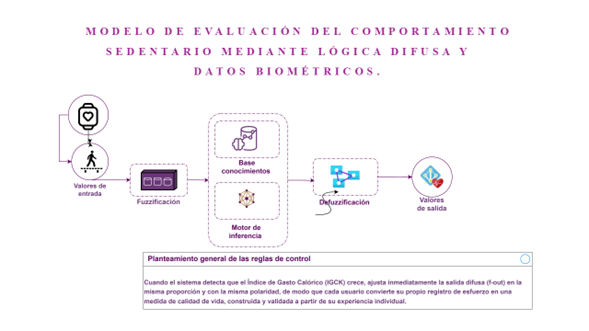
\includegraphics[width=0.95\textwidth]{figuras/diagrama_de_tesis.png}
    \caption{Arquitectura del sistema de clasificaci├│n de sedentarismo mediante l├│gica difusa}
    \label{fig:diagrama_tesis}
\end{figure}
